\chapter{Plotting data}
\label{ch:plotting}

A picture says more than a thousand words and nowhere is this more
true than in statistics. So before we explore the more quantitative
aspects of data analysis, it is useful to \emph{visualise} the data.
Consider, for example, the following four bivariate datasets
(Anscombe's quartet\footnote{Anscombe, F.J., 1973. Graphs in
  statistical analysis. \emph{The American statistician}, 27(1),
  pp.17-21.}):\medskip

\noindent\begin{minipage}[t][][b]{.6\textwidth}
  \begin{tabular}{cc|cc|cc|cc}
    \multicolumn{2}{c}{I} & \multicolumn{2}{c}{II} &
    \multicolumn{2}{c}{III} & \multicolumn{2}{c}{IV} \\
    $x$ & $y$ & $x$ & $y$ & $x$ & $y$ & $x$ & $y$ \\ \hline
    10.0 & 8.04 & 10.0 & 9.14 & 10.0 & 7.46 & 8.0 & 6.58 \\
    8.0 & 6.95 & 8.0 & 8.14 & 8.0 & 6.77 & 8.0 & 5.76 \\
    13.0 & 7.58 & 13.0 & 8.74 & 13.0 & 12.74 & 8.0 & 7.71 \\
    9.0 & 8.81 & 9.0 & 8.77 & 9.0 & 7.11 & 8.0 & 8.84 \\
    11.0 & 8.33 & 11.0 & 9.26 & 11.0 & 7.81 & 8.0 & 8.47 \\
    14.0 & 9.96 & 14.0 & 8.10 & 14.0 & 8.84 & 8.0 & 7.04 \\
    6.0 & 7.24 & 6.0 & 6.13 & 6.0 & 6.08 & 8.0 & 5.25 \\
    4.0 & 4.26 & 4.0 & 3.10 & 4.0 & 5.39 & 19.0 & 12.50 \\
    12.0 & 10.84 & 12.0 & 9.13 & 12.0 & 8.15 & 8.0 & 5.56 \\
    7.0 & 4.82 & 7.0 & 7.26 & 7.0 & 6.42 & 8.0 & 7.91 \\
    5.0 & 5.68 & 5.0 & 4.74 & 5.0 & 5.73 & 8.0 & 6.89 \\
  \end{tabular}
\end{minipage}
\begin{minipage}[t][][t]{.4\textwidth}
  \captionof{table}{Anscombe's quartet of bivariate data pairs.}
  \label{tab:anscombe}
\end{minipage}\medskip

For all four datasets (I -- IV):

\begin{itemize}\label{pg:anscombe}
\item the mean (see Chapter~\ref{ch:summary-statistics}) of $x$ is 9
\item the variance (see Chapter~\ref{ch:summary-statistics}) of $x$ is 11
\item the mean of $y$ is 7.50
\item the variance of $y$ is 4.125
\item the correlation coefficient (see Chapter~\ref{ch:regression})
  between $x$ and $y$ is 0.816
\item the best fit line (see Chapter~\ref{ch:regression}) is given by $y =
  3.00 + 0.500 x$
\end{itemize}

So from a numerical point of view, it would appear that all four
datasets are identical. However, when we visualise the data as
bivariate scatter plots, they turn out to be very different:\medskip

\noindent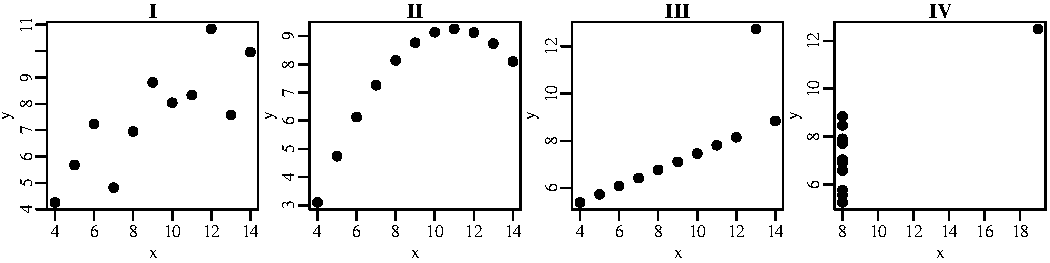
\includegraphics[width=\textwidth]{../figures/anscombe.pdf}
\begingroup
\captionof{figure}{Anscombe's quartet shown as bivariate scatter
  plots.\medskip}\label{fig:anscombe}
\endgroup

Bivariate scatter plots are just one way to visualise analytical data.
Many other graphical devices exist, each of which is appropriate for a
particular type of data. The following sections of this chapter will
introduce a number of these data types, and the associated plots.

\section{Discrete data}
\label{sec:discrete}

Some geological datasets take on discrete values and can be visualised
as bar charts or histograms. We can distinguish between three such
types of data.

\begin{enumerate}

\item\textbf{Categorical} data take on a limited number of values,
  assigning each `object' to a particular \emph{unordered} class or
  category. Geological examples of categorical data include animal
  species in a bone bed; the modal composition of a thin section; and
  lithologies in a mapping area. Figure~\ref{fig:discrete}.a shows a
  dataset of 41 clast counts in a river bed:
  \begin{center}
    \begin{tabular}{cccc}
      granite & basalt & gneiss & quartzite \\ \hline
      10 & 5 & 6 & 20  
    \end{tabular}
  \end{center}

\item\textbf{Ordinal} data are a special type of categorical data, in
  which the classes are \emph{ordered} but the distances between them
  are either irregular or unknown. Geological examples of ordinal
  quantities include Moh's hardness scale; metamorphic grade; and the
  geologic timescale. Figure~\ref{fig:discrete}.b tallies the relative
  areas (normalised to 100\%) covered by rocks of different
  biostratigraphic age, in Germany:
  \begin{center}
    \begin{tabular}{ccccc}
      Precambrian & Palaeozoic & Mesozoic & Tertiary & Quaternary\\ \hline
      6.6\% & 16.9 \% & 29.4\% & 7.2\% & 39.9\%
    \end{tabular}
  \end{center}

\item\textbf{Count} data are a special type of ordinal data in which
  the categories are evenly spaced into integer intervals. Geological
  examples of count data include the number of gold chips found in a
  panning session; the annual number of earthquakes that exceed a
  certain magnitude; and the number of dry wells in a wildcat drilling
  survey. Figure~\ref{fig:discrete}.c shows the number of discovery
  wells in 160 equally sized tracts of the Permian Basin in Texas:
  \begin{center}
    \begin{tabular}{c|ccccccc}
     \# wells & 0 & 1 & 2 & 3 & 4 & 5 & 6 \\ \hline
     \# tracts & 70 & 42 & 26 & 17 & 3 & 1 & 1
    \end{tabular}
  \end{center}

\end{enumerate}

\noindent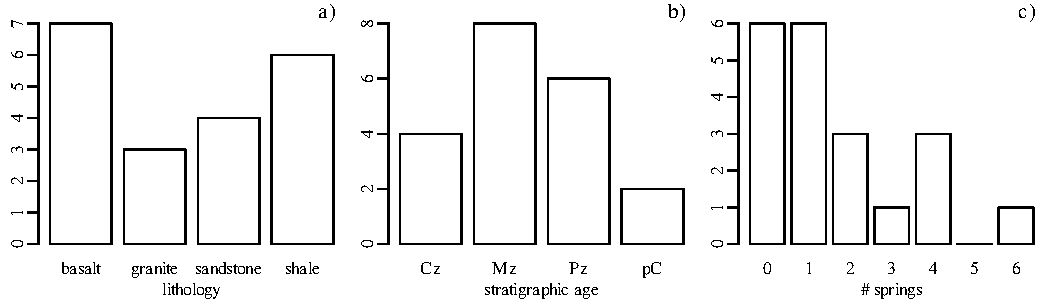
\includegraphics[width=\textwidth]{../figures/discrete.pdf}\medskip
\begingroup \captionof{figure}{Examples of discrete datasets, shown as
  bar charts. a) Categorical dataset of 41 random clast counts in a
  river bed. The order of the categories along the horizontal axis is
  completely arbitrary and can be changed without loss of
  information. b) Ordinal dataset summarising the surficial geology of
  Germany, expressed as the total percentage of areas covered by
  Precambrian (pC), Palaeozoic (Pz), Mesozoic (Mz), Tertiary (T) and
  Quaternary (Q) rocks. These five categories are listed in
  chronological order, but span vastly different lengths of time; c)
  The number of discovery wells per tract in an area of the Permian
  Basin (Texas) that was subdivided into 168 equally sized quadrats.}
\label{fig:discrete}
\endgroup

\section{Continuous data}
\label{sec:continuous}

Not all geological or geophysical measurements take on discrete
values.  Many are free to take on decimal values. We can also
subdivide these continuous data into further classes, such as:

\begin{enumerate}
\item\textbf{Cartesian quantities}\footnote{The terms Cartesian and
Jeffreys quantities were coined by Mosegaard and Tarantola (2002,
doi:10.1016/S0074-6142(02)80219-4), in honour of French mathematician
Ren\'{e} Descartes and British geophysicist Sir Harold Jeffreys. They
are also referred to as balances and amounts, respectively, by
Mosteller and Tukey (1977, ISBN:0-201-04854-X).\label{ftn:Tarantola}}
  can have any decimal value, including positive and negative
  ones. Geoscientific examples of this data type include the magnitude
  of earthquakes; the spontaneous electrical potential between
  geological strata; or the pH of aqueous
  solutions. Figure~\ref{fig:continuous}.a shows a dataset with pH
  measurements in 20~samples of rain water:
  \begin{center}
    6.2, 4.4, 5.6, 5.2, 4.5, 5.4, 4.8, 5.9, 3.9, 3.8, 5.1, 4.1, 5.1, 5.5,
    5.1, 4.6, 5.7, 4.6, 4.6, 5.6
  \end{center}
\item\textbf{Jeffreys quantities}\textsuperscript{\ref{ftn:Tarantola}}
  can only have positive values. Examples of this include mass,
  volume, density, speed, etc. Figure~\ref{fig:continuous}.b shows 20
  sedimentary clast size measurements, in centimetres:
  \begin{center}
    0.35, 11.00, 6.00, 1.80, 2.30, 0.59, 8.40, 2.90, 5.90, 2.10,\\
    1.20, 2.10, 1.10, 1.60, 0.90, 1.70, 3.40, 0.53, 2.20, 7.70
  \end{center}
\item\textbf{Proportions} are quantities that are constrained to a
  finite interval from 0 to 1 (or from 0 to 100\%). Examples of this
  include chemical concentrations; volume fractions; and porosities.
  Figure~\ref{fig:continuous}.c shows a dataset of twenty porosity
  measurements in limestone:
  \begin{center}
    0.058, 0.28, 0.12, 0.27, 0.40, 0.12, 0.038, 0.063, 0.17, 0.16,\\
    0.95, 0.94, 0.92, 0.88, 0.88, 0.70, 0.92, 0.72, 0.74, 0.84
  \end{center}
\end{enumerate}

\noindent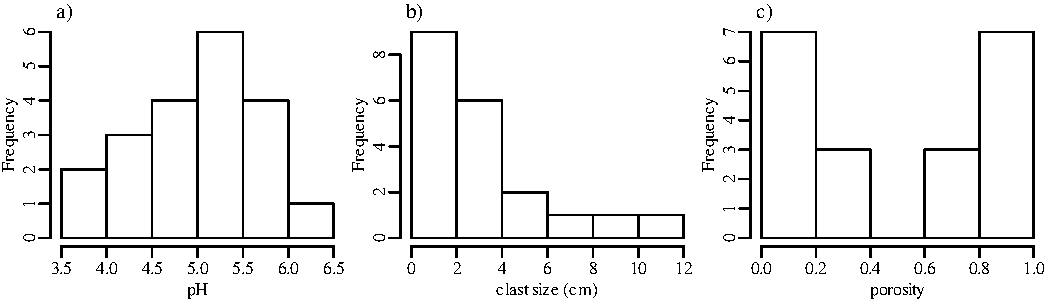
\includegraphics[width=\textwidth]{../figures/continuous.pdf}\medskip
\begingroup \captionof{figure}{Three continuous datasets, shown as
  histograms. a) pH measurements of river water (free to take on
  positive and negative values); b) clast size measurements
  (non-negative numbers); and c) porosity measurements of limestone
  (values between 0 and 1).}
\label{fig:continuous}
\endgroup

\section{Histograms}\label{sec:histogram}

The discrete values of Section~\ref{sec:discrete} naturally fall into
bins and the most obvious way to visualise them is as bar charts.
Likewise, the continuous data of Section~\ref{sec:continuous} can also
be collected into bins and plotted as histograms. However, this
binning exercise poses two practical problems.

\begin{enumerate}

\item\textbf{How many bins should be used, and how wide should they be?}

  The number of bins strongly affects the appearance of a histogram.
  Figure~\ref{fig:binwidth} shows the pH data on two histograms with
  the individual measurements marked as vertical ticks
  underneath. This is also known as a \emph{rug plot}, and allows us
  to better assess the effect of bin width on the appearance of
  histograms:
  
  \noindent\begin{minipage}[t][][b]{.55\linewidth}
  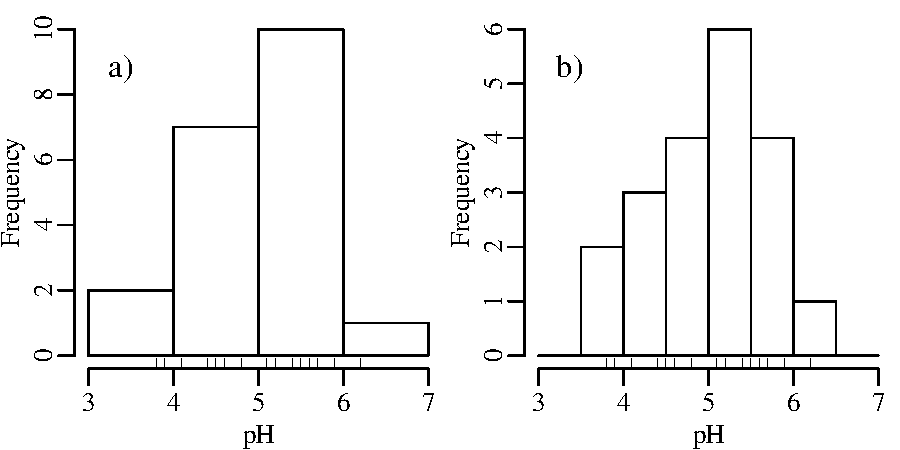
\includegraphics[width=\textwidth]{../figures/binwidth.pdf}\medskip
  \end{minipage}
  \begin{minipage}[t][][t]{.45\linewidth}
    \captionof{figure}{Histogram a) uses a bin width of 1~pH unit
      whereas histogram b) uses a bin width of 0.5~pH units. The two
      histograms look considerably different and it is not immediately
      clear which choice of bin width is best.}
    \label{fig:binwidth}
  \end{minipage}

  A number of rules of thumb are available to choose the optimal number
  of bins. For example, \texttt{Excel} uses a simple square root rule:

  \begin{equation}
    \mbox{\#{bins} = } \sqrt{n}
  \end{equation}

  \noindent where $n$ is the number of observations (i.e. $n = 20$ for
  the pH example). \texttt{R} uses Sturges' Rule:

  \begin{equation}
    \mbox{\#{bins} = } \log_2(n) + 1
  \end{equation}

  \noindent however no rule of thumb is optimal in all situations.

\item\textbf{Where to place the bins?}

Even when the number of bins has been fixed, just shifting them
slightly to the left or to the right can have a significant effect on
the appearance of the histogram. For example:

\noindent\begin{minipage}[t][][b]{.55\linewidth}
  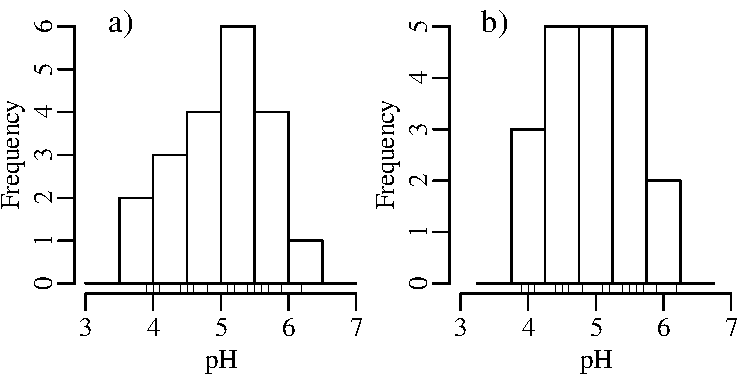
\includegraphics[width=\textwidth]{../figures/binpos.pdf}\medskip
\end{minipage}
\begin{minipage}[t][][t]{.45\linewidth}
  \captionof{figure}{Two histograms of the pH data whose bin widths
    are the same, but whose bins have been offset by 0.25 pH units.
    This arbitrary decision strongly affects the appearance of the
    histogram.}
  \label{fig:binpos}
\end{minipage}

\end{enumerate}

\section{Kernel density estimation}\label{sec:KDE}

To solve the bin placement problem, let us explore a variant of the
ordinary histogram that is constructed as follows:
\begin{enumerate}
\item Rank the measurements from low to high along a line.
\item Place a rectangular `box' on top of each measurement.
\item Stack the boxes to create one connected line.
\end{enumerate}
\noindent\begin{minipage}[t][][b]{.3\textwidth}
  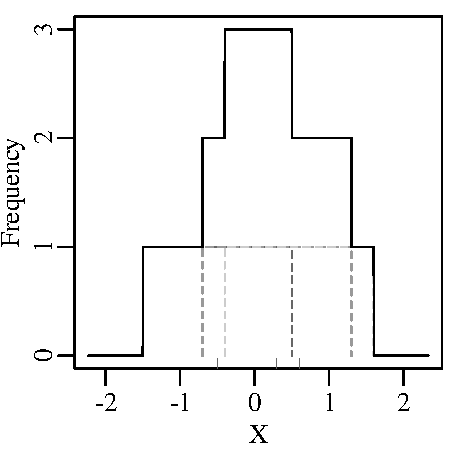
\includegraphics[width=\textwidth]{../figures/rectKDE.pdf}\medskip
\end{minipage}
\begin{minipage}[t][][t]{.7\textwidth}
  \captionof{figure}{The rug plot along the bottom axis represents
    three data points. The grey dashed lines mark rectangular boxes
    (`kernels') that are centred around each of these data points. The
    black step function is obtained by taking the sum of these
    boxes. This procedure removes the need to choose bin locations.}
  \label{fig:rectangles}
\end{minipage}

Normalising the area under the resulting curve produces a so-called
Kernel Density Estimate (KDE). The mathematical definition of this
function is:

\begin{equation}
  KDE(x) = \frac{1}{nh} \sum\limits_{i=1}^{n} K\!\left(\frac{x-x_i}{h}\right)
\end{equation}

\noindent where $x_i$ is the $i$\textsuperscript{th} measurement (out
of $n$), $h$ is the `bandwidth' of the kernel density estimator, and
$K(u)$ is the `kernel' function. For the rectangular kernel:

\begin{equation}
  K(u) = 1/2 \mbox{~if~}|u| \leq 1, \mbox{~and~} K(u) = 0 \mbox{~otherwise}
\end{equation}

Applying this method to the pH data:

\noindent\begin{minipage}[t][][b]{.3\textwidth}
  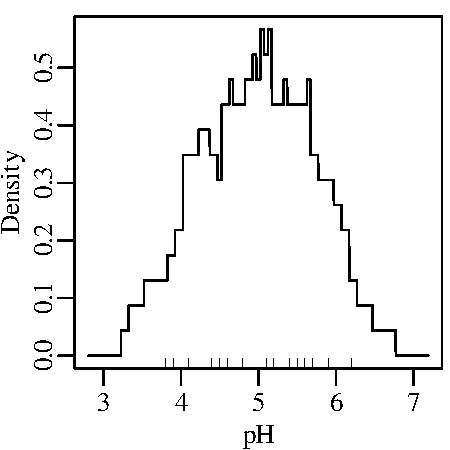
\includegraphics[width=\textwidth]{../figures/pHrectKDE.pdf}\medskip
\end{minipage}
\begin{minipage}[t][][t]{.7\textwidth}
  \captionof{figure}{Rectangular KDE of the pH data, constructed using
    the same procedure as shown in Figure~\ref{fig:rectangles}. The
    area under this curve has been normalised to unity.}
  \label{fig:pHrectKDE}
\end{minipage}

Instead of a rectangular kernel, we could also use triangles to
construct the KDE curve, or any other (symmetric) function. One
popular choice is the Gaussian function:

\begin{equation}
  K(u) = \frac{1}{\sqrt{2\pi}}\exp\!\left[-\frac{u^2}{2}\right]
  \label{eq:gaussiankernel}
\end{equation}

\noindent which produces a continuous KDE function:\medskip

\noindent\begin{minipage}[t][][b]{.3\textwidth}
  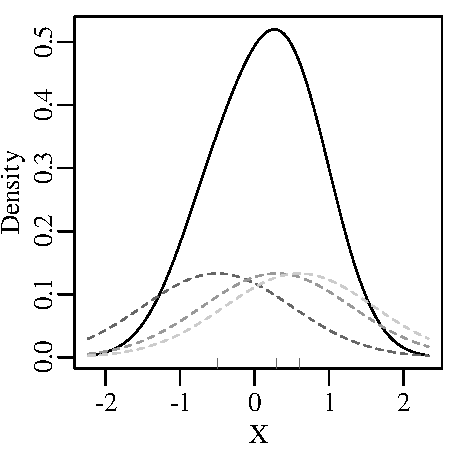
\includegraphics[width=\textwidth]{../figures/gaussKDE.pdf}\medskip
\end{minipage}
\begin{minipage}[t][][t]{.7\textwidth}
  \captionof{figure}{Using a Gaussian kernel instead of a rectangular
    kernel on the three data points of Figure~\ref{fig:rectangles}.
    This produces a smooth KDE.}
\end{minipage}

Using the Gaussian kernel to plot the pH data:\medskip

\noindent\begin{minipage}[t][][b]{.3\textwidth}
  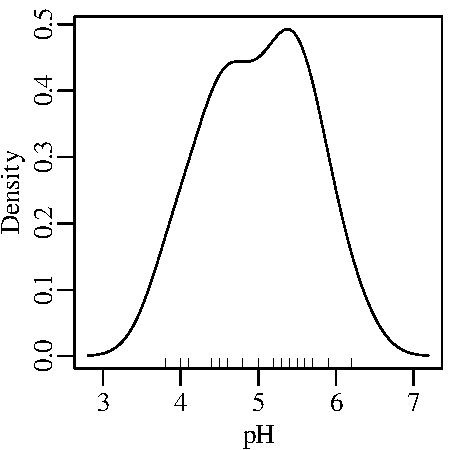
\includegraphics[width=\textwidth]{../figures/pHgaussKDE.pdf}\medskip
\end{minipage}
\begin{minipage}[t][][t]{.7\textwidth}
  \captionof{figure}{Gaussian KDE of the pH data. The continuous curve
    does more justice to the continuous data than the discrete step
    function of Figures~\ref{fig:binwidth}, \ref{fig:binpos} or
    \ref{fig:pHrectKDE}.}
  \label{fig:pHgaussKDE}
\end{minipage}

Although kernel density estimation solves the bin placement problem,
it is not entirely free of design decisions. The bandwidth $h$ of a
KDE fulfils a similar role as the bin width of a histogram. Changes in
$h$ affect the \emph{smoothness} of the KDE curve:\medskip

\noindent\begin{minipage}[t][][b]{.6\textwidth}
  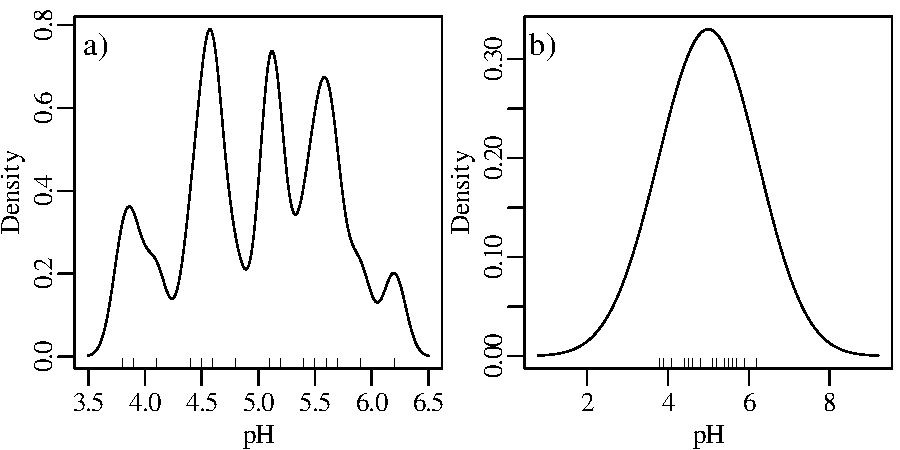
\includegraphics[width=\textwidth]{../figures/bandwidth.pdf}\medskip
\end{minipage}
\begin{minipage}[t][][t]{.4\textwidth}
  \captionof{figure}{KDEs of the pH data with a) a kernel bandwidth of
    $h=0.1$; and b) a bandwidth of $h=1$. Using a narrow bandwidth
    undermooths the data, whereas a wide bandwidth produces an
    oversmoothed distribution.}
\end{minipage}

Bandwidth selection is a similar problem to bin width selection.  A
deeper discussion of this problem falls outside the scope of text.
Suffice it to say that most statistical software (including $R$) use
equivalent rules of thumb to Sturges' Rule to set the bandwidth.  But
these values can be easily overruled by the user.

\section{Data transformations}
\label{sec:transformations}

As discussed in Section~\ref{sec:continuous}, interval data such as
the clast sizes of Figure~\ref{fig:continuous}.b exist within an
infinite half space between 0 and $+\infty$. However, when we
visualise them as a KDE, the left tail of this curve may extend into
negative data space, implying that there is a finite chance of
observing negative clast sizes:

\noindent\begin{minipage}[t][][b]{.3\textwidth}
  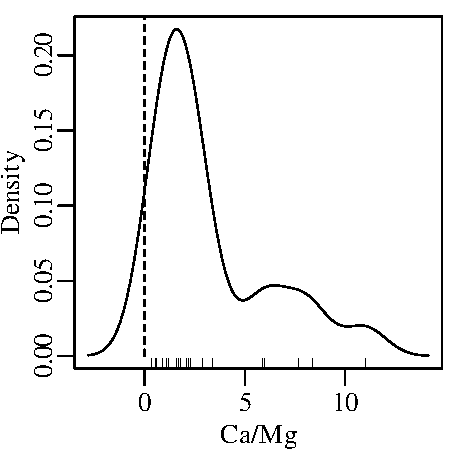
\includegraphics[width=\textwidth]{../figures/negativeKDE.pdf}\medskip
\end{minipage}
\begin{minipage}[t][][t]{.7\textwidth}
  \captionof{figure}{KDE of 20 clast size measurements.  Even though
    all the measurements are strictly positive, the curve extends into
    negative data space.}
  \label{fig:negativeKDE}
\end{minipage}

This problem can be solved by transforming the interval data to the
entire infinite space of numbers by applying a logarithmic
transformation:
\begin{equation}
  u = \ln[x]
\end{equation}

After constructing the KDE, the results can then be mapped back to
linear space using an exponential transformation:
\begin{equation}
  x = \exp[u]
\end{equation}

\noindent\begin{minipage}[t][][b]{.6\textwidth}
  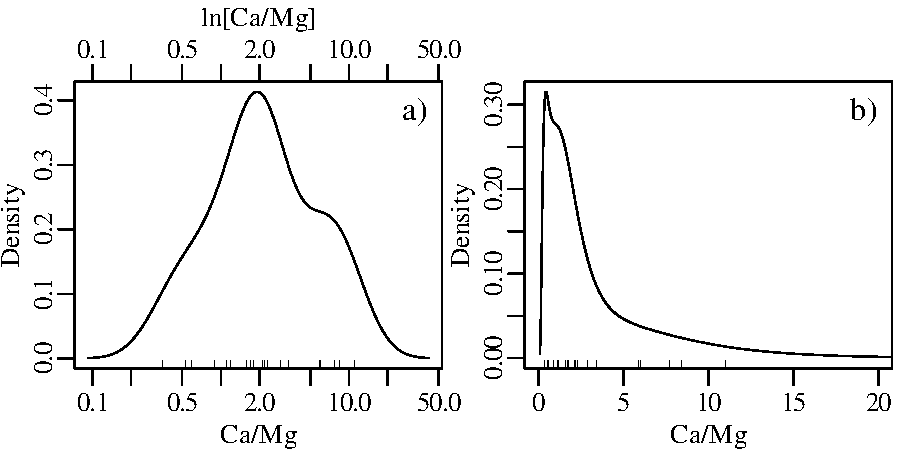
\includegraphics[width=\textwidth]{../figures/logKDE.pdf}\medskip
\end{minipage}
\begin{minipage}[t][][t]{.4\textwidth}
  \captionof{figure}{a) KDE of the clast size measurements, after
    applying a logarithmic transformation.  Note how the distribution
    has become more symmetric compared to the linear scale of
    Figure~\ref{fig:negativeKDE}. b) The same KDE mapped back to
    linear scale. Unlike Figure~\ref{fig:negativeKDE}, the mapped
    distribution does not cross over into negative values.}
  \label{fig:logKDE}
\end{minipage}

Interval data are just one example of constrained measurements.  As
another example, consider the porosity data of
Figure~\ref{fig:continuous}.c. Again, the Gaussian KDE of the data
plots into physically impossible values of $<0$ and $>1$:\medskip

\noindent\begin{minipage}[t][][b]{.3\textwidth}
  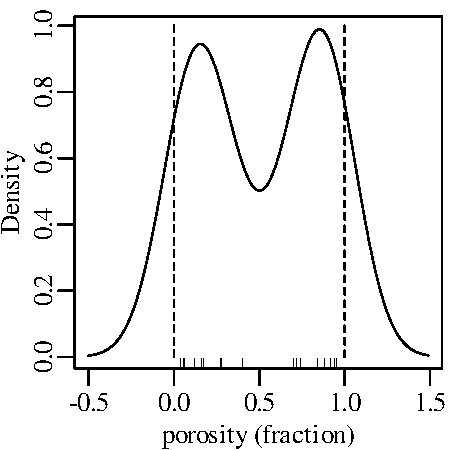
\includegraphics[width=\textwidth]{../figures/porosityKDE.pdf}\medskip
\end{minipage}
\begin{minipage}[t][][t]{.7\textwidth}
  \captionof{figure}{KDE of 20 porosity measurements.  Even though all
    the measurements are between 0 and 1, the KDE extends beyond these
    hard limits.}
  \label{fig:porosityKDE}
\end{minipage}

Using a similar approach as before, the dataspace can be opened up
from the constraints of the 0 to 1 interval to the entire line of
numbers, from $-\infty$ to $+\infty$. For proportions, this is
achieved by the \emph{logistic transformation}:

\begin{equation}
  u = \mbox{logit}(x) = \ln\!\left[\frac{x}{1-x}\right]
  \label{eq:logit}
\end{equation}

After constructing the density estimate (or carrying out any other
numerical manipulation), the results can be mapped back to the 0 to 1
interval with the inverse logit transformation:

\begin{equation}
  x = \mbox{logit}^{-1}(u) = \frac{\exp[u]}{\exp[u]+1}
  \label{eq:invlogit}
\end{equation}

\noindent\begin{minipage}[t][][b]{.6\textwidth}
  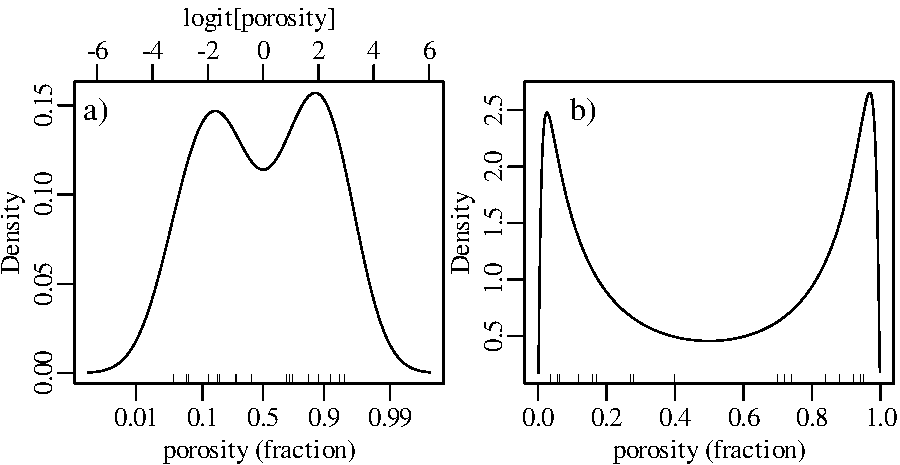
\includegraphics[width=\textwidth]{../figures/logitKDE.pdf}\medskip
\end{minipage}
\begin{minipage}[t][][t]{.4\textwidth}
  \captionof{figure}{a) KDE of the porosity data, after applying a
    logistic transformation.  Note the two horizonal axes.  The top
    axis marks the transformed values on a linear scale that extends
    from $-\infty$ to $+\infty$. The bottom axis is labeled by the
    actual porosity values on a non-linear scale that extends from 0
    to 1. b) The same distribution mapped back to the 0 -- 1
    interval.}
  \label{fig:logitKDE}
\end{minipage}

We will see in Chapter~\ref{ch:compositional} that the logistic
transformation is a special case of a general class of \emph{logratio
  transformations} that are useful for the analysis of
\emph{compositional data}.

\section{Multivariate distributions}
\label{sec:multivariate}

KDEs can be generalised from one to two dimensions.  For example,
consider a dataset of eruption timings from the Old Faithful geyser in
Yellowstone national park (Wyoming, USA): \medskip

\noindent\begin{minipage}[t][][b]{.5\textwidth}
  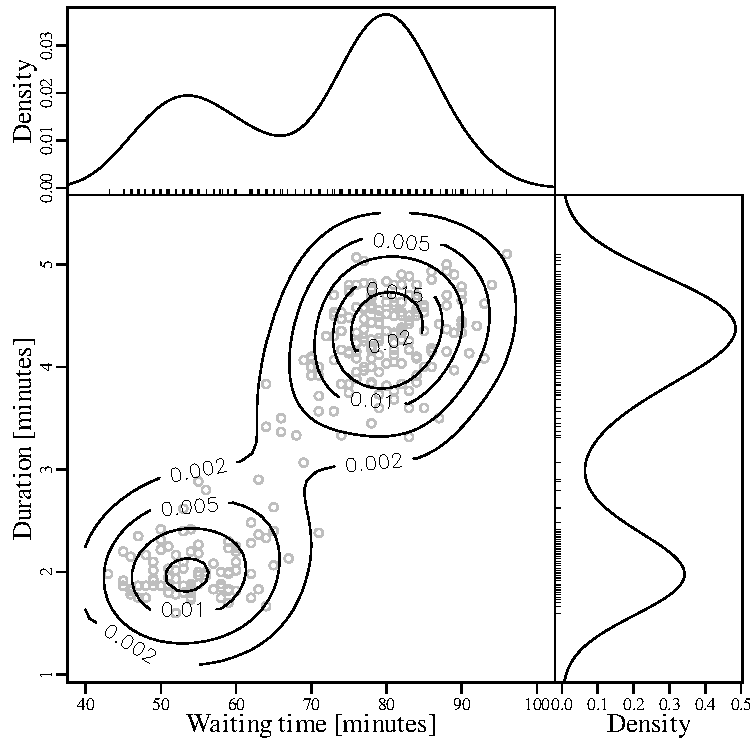
\includegraphics[width=\textwidth]{../figures/KDE2D.pdf}\medskip
\end{minipage}
\begin{minipage}[t][][t]{.5\textwidth}
  \captionof{figure}{Old Faithful eruption measurements. The dataset
    records 272 observations of 2 variables: the duration of each
    eruption, and the waiting time between them. Both variables are
    expressed in minutes. The lower left panel shows the bivariate
    measurements as grey circles. The contour lines represent a
    2-dimensional KDE. The marginal distributions of the waiting times
    (top) and eruption durations (right) are shown as 1-dimensional
    KDEs.}
  \label{fig:KDE2D}
\end{minipage}

It is generally not possible to visualise datasets of more than two
dimensions in a single graphic. In this case there are two options:

\begin{enumerate}
  \item plot the data as a series of 1- or 2-dimensional marginal
    plots; or
  \item extract the most important patterns or trends in the data by
    projection onto a lower dimensional plane. Then show these
    projected data as a lower dimensional graphic.
\end{enumerate}

The second strategy is also known as ``ordination'' and will be
discussed in detail in Section~\ref{sec:PCA}.

\section{Empirical cumulative distribution functions}
\label{sec:ECDF}

Both histograms and kernel density estimates require the selection of
a `smoothing parameter'. For the histogram, this is the bin width; for
the KDE, it is the bandwidth. Despite the existence of rules thumbs to
automatically choose an appropriate value for the smoothing parameter,
there nevertheless is a level of arbitrariness associated with
them. The empirical cumulative distribution function (ECDF) is an
alternative data visualisation device that does not require
smoothing. An ECDF is step function that jumps up by $1/n$ at each of
$n$ data points.  The mathematical formula for this procedure can be
written as:
  
  \begin{equation}
    F(x) = \sum\limits_{i=1}^{n} 1(x_i<x)/n
    \label{eq:ECDF}
  \end{equation}
 
\noindent where $1(\ast) = 1$ if $\ast$ is `true' and $1(\ast) = 0$ if
$\ast$ is `false'. The y-coordinates of the ECDF are values from 0 to
1 that mark the fraction of the measurements that are less than a
particular value.  Plotting the pH, clast size, porosity and geyser
data as ECDFs:

\noindent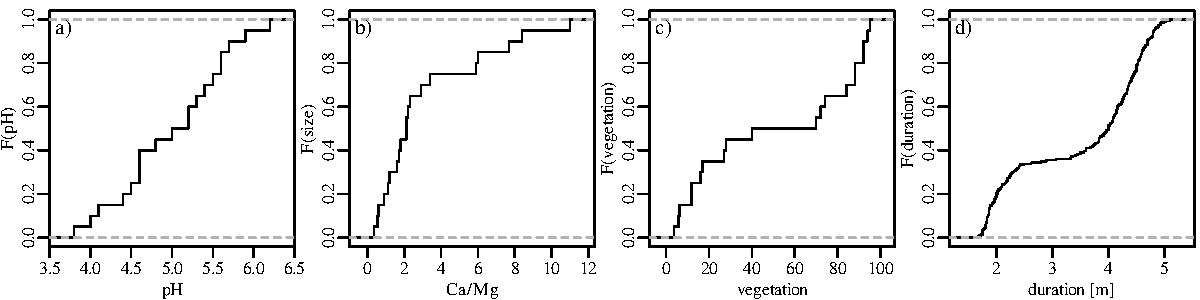
\includegraphics[width=\textwidth]{../figures/ECDFs.pdf}
\begingroup
\captionof{figure}{Empirical cumulative distribution functions (ECDFs)
  of, from left to right: a) the pH data (whose KDE is shown in
  Figure~\ref{fig:pHgaussKDE}); b) the clast size data of
  Figure~\ref{fig:negativeKDE}; c) the porosity data of
  Figure~\ref{fig:porosityKDE}; and d) the eruption time data of
  Figure~\ref{fig:KDE2D}. Note that ECDFs are only applicable to
  1-dimensional datasets.\medskip}
\label{fig:ECDFs}
\endgroup

ECDFs do not require binning or selecting a bandwidth.  Because they
do not require smoothing, they do not spill over into physically
impossible values for the clast size and porosity data. Therefore the
construction of an ECDF is completely hands off.\medskip

The visual interpetation of ECDFs is different from that of histograms
or KDEs. Whereas different clusters of values stand out as `peaks' in
a histogram or KDE, they are marked by steep segments of the ECDF. For
example, the two peaks in the KDE of the geyser data
(Figure~\ref{fig:KDE2D}) correspond to two steps in the ECDF
(Figure~\ref{fig:ECDFs}.d).
